\section{Gjennomføring med måleresultater}

\subsection{Måling på RC-ledd}
\subsubsection{Én kondensator}
Signalgeneratoren ble stilt inn på $f=150\text{Hz}$ og amplituden målte $1.0\text{V{p-p}}$ på oscilloskopet.

\begin{figure}[H]
\centering
\begin{circuitikz}[american voltages]

    \node[circle, fill=black, inner sep=1.2pt] (A)  at (0,0) {};
    \node[circle, fill=black, inner sep=1.2pt] (B)  at (0,4) {};
    \node[circle, fill=black, inner sep=1.2pt] (C)  at (8,4) {};
    \node[circle, fill=black, inner sep=1.2pt] (D)  at (8,0) {};

    \node at (A) [ground] {};
    \node at (D) [ground] {};
    \node[above left] at (B) {$A$};
    \node[above right] at (C) {$B$};
    \node[above right] at (D) {$C$};

    \draw (A) to[sV, l_=$V_1$] (B);
    \draw (B) to[R, l_=$R_4$, a^=$1\text{k}\Omega$] (C);
    \draw (C) to[C, l_=$C_7$, a^=$470\text{nF}$] (D);

\end{circuitikz}
\caption{Krets for måling av RC-ledd.}
\end{figure}

\noindent
Vi målte spenning over kondensatoren $C_7$ på kanal 1 på oscilloskopet, og spenningen over både motstanden $R_4$ og kondensatoren $C_7$ på kanal 2. Det betyr at kanal 1 var parallellkoblet gjennom node $B$ og $C$, og kanal 2 var koblet gjennom node $A$ og $C$. Begge kanaler er i DC-modus. Resultatet av disse to grafene blir som vist i figur~\ref{fig:rc_ledd_alene}.

\begin{figure}[H] % eller [htbp] hvis du bruker float-pakken lite
    \centering
    \includegraphics[width=0.7\textwidth]{Media/alene-C.jpeg}
    \caption{Alene kondensator.}
    \label{fig:rc_ledd_alene}
\end{figure}





\paragraph{Spenningen over motstanden $R_4$. } For å kunne måle spenningen over denne motstanden må vi gjøre om på kretsen for å unngå å måle over ingen spenningsforskjell. Kretsen blir nå seende slik ut.
\begin{figure}[H]
\centering
\begin{circuitikz}[american voltages]

    \node[circle, fill=black, inner sep=1.2pt] (A)  at (0,0) {};
    \node[circle, fill=black, inner sep=1.2pt] (B)  at (0,4) {};
    \node[circle, fill=black, inner sep=1.2pt] (C)  at (8,4) {};
    \node[circle, fill=black, inner sep=1.2pt] (D)  at (8,0) {};

    \node at (A) [ground] {};
    \node at (D) [ground] {};
    \node[above left] at (B) {$A$};
    \node[above right] at (C) {$B$};
    \node[above right] at (D) {$C$};

    \draw (A) to[sV, l_=$V_1$] (B);
    \draw (C) to[R, l_=$R_4$, a^=$1\text{k}\Omega$] (D);
    \draw (B) to[C, l_=$C_7$, a^=$470\text{nF}$] (C);

\end{circuitikz}
\caption{Krets for måling av RC-ledd.}
\end{figure}

\noindent
Nå kan det måles mellom node $B$ og $C$. Resultatet på oscilloskopet ble seende slik ut.

\begin{figure}[H] % eller [htbp] hvis du bruker float-pakken lite
    \centering
    \includegraphics[width=0.7\textwidth]{Media/spenning_R4.jpeg}
    \caption{Parallellkoblet kondensatorer.}
    \label{fig:spenning_R4}
\end{figure}


Grafen kan forklares med å se på strømmen gjennom den. Siden spenningen over motsatnden beskrives som $V_R(t)$ = $R_4i(t)$. I et RC-ledd vil strømmen bestemmes av derivert spenning over kondensatoren:
\[
\begin{aligned}
    i(t)&=C\frac{dv_C(t)}{dt} \\
    v_R(t)&=RC\frac{dv_C(t)}{dt}
\end{aligned}
\]
\noindent
Nå kan vi se at spenningen over motstanden bestemmes av endringen i spenningen i kondensatoren. Derfor vil det bli stor spenning over motstanden når kondensatorspenningen stiger eller faller raskt. Når spenningen over kondensatoren flater ut vil derfor $V_R(t)$ eksponentielt synke mot null. Vi kan grafe $V_C(t)$, $V_1(t)$ og $V_R(t)$ for å se forholdet mellom dem. Ved å bruke de kjente verdiene og sette dem inn i ligning~\ref{eq:spenning_i_kondensator}.

\[
\tau = R_4 \cdot C_7 = 0.470\text{ms}
\]
\[
V_F = 1.0\text{V}
\]

\[
\begin{aligned}
v_C(t) &=
\begin{cases}
1 -  e^{-{t}/{0.470\text{ms}}}, 
    & 0 \le t \le 10\text{ms},\\[0.5em]
e^{-\left(t - 10\text{ms}\right)/{0.470\text{ms}}}, 
    & 10\text{ms} \le t \le 20\text{ms},
\end{cases}
\end{aligned}
\]

\[
v_R(t) = R_4C_7\cdot v_C'(t)
\]

\[
\begin{aligned}
v_R(t) &=
\begin{cases}
e^{-{t}/{0.470\text{ms}}}, 
    & 0 \le t \le 10\text{ms},\\[0.5em]
-e^{-\left(t - 10\text{ms}\right)/{0.470\text{ms}}}, 
    & 10\text{ms} \le t \le 20\text{ms},
\end{cases}
\end{aligned}
\]


\begin{figure}[H]
\centering
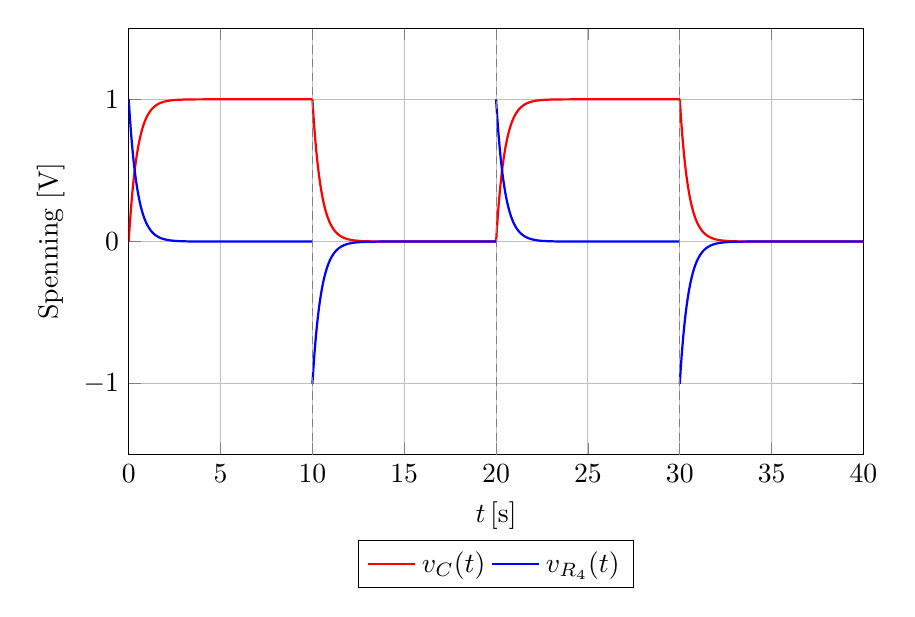
\begin{tikzpicture}
\begin{axis}[
    width=0.9\textwidth,
    height=7cm,
    xlabel={$t\,[\mathrm{s}]$},
    ylabel={Spenning\ [V]},
    xmin=0, xmax=40,
    ymin=-1.5, ymax=1.5,
    grid=both,
    legend style={at={(0.5,-0.2)},anchor=north,legend columns=2},
    samples=200
]

    % --- v_C(t): spenning over kondensatoren ---
    % Periode 1: 0–20 s
    \addplot[
        thick,
        red,
        domain=0:10
    ]
        {(1 - exp(-x/0.470))};
    \addplot[
        thick,
        red,
        domain=10:20,
        forget plot
    ]
        {exp(-(x-10)/0.470)};
    % Periode 2: 20–40 s
    \addplot[
        thick,
        red,
        domain=20:30,
        forget plot
    ]
        {(1 - exp(-(x - 20)/0.470))};
    \addplot[
        thick,
        red,
        domain=30:40,
        forget plot
    ]
        {exp(-(x-30)/0.470)};
    \addlegendentry{$v_C(t)$}

    % --- v_R4(t): spenning over motstanden R4 ---
    % Periode 1: 0–20 s
    \addplot[
        thick,
        blue,
        domain=0:10
    ]
        {exp(-x/0.470)};
    \addplot[
        thick,
        blue,
        domain=10:20,
        forget plot
    ]
        {-exp(-(x-10)/0.470)};
    % Periode 2: 20–40 s
    \addplot[
        thick,
        blue,
        domain=20:30,
        forget plot
    ]
        {exp(-(x-20)/0.470)};
    \addplot[
        thick,
        blue,
        domain=30:40,
        forget plot
    ]
        {-exp(-(x-30)/0.470)};
    \addlegendentry{$v_{R_4}(t)$}

    % Vertikale hjelpelinjer (valgfritt, ikke i legend)
    \addplot[
        gray,
        densely dashed,
        forget plot
    ]
        coordinates {(10,-1.5) (10,1.5)};
    \addplot[
        gray,
        densely dashed,
        forget plot
    ]
        coordinates {(20,-1.5) (20,1.5)};
    \addplot[
        gray,
        densely dashed,
        forget plot
    ]
        coordinates {(30,-1.5) (30,1.5)};

\end{axis}
\end{tikzpicture}
\caption{Teoretisk spenning over kondensatoren $C_T$ og motstanden $R_4$ for et firkantet inngangssignal med periode $20\,\text{s}$ og tidskonstant $\tau = 0{,}47\,\text{s}$.}
\end{figure}

\noindent
Siden dette er teoretisk tilnærming med verdiene vi har er ikke grafen helt lik den på oscilloskopet. Uansett, så bekrefter den at grafene henger sammen. Utledningen av at spenningen over motstanden er proporsjonal med endringen i spenningen på kondensatoren stemmer overens med grafen.













\subsubsection{To kondensatorer i serekobling}

\begin{figure}[H]
\centering
\begin{circuitikz}[american voltages]

    \node[circle, fill=black, inner sep=1.2pt] (A)  at (0,0) {};
    \node[circle, fill=black, inner sep=1.2pt] (B)  at (0,4) {};
    \node[circle, fill=black, inner sep=1.2pt] (C)  at (8,4) {};
    \node[circle, fill=black, inner sep=1.2pt] (D)  at (8,0) {};

    \node at (A) [ground] {};
    \node at (D) [ground] {};
    \node[above left] at (B) {$A$};
    \node[above right] at (C) {$B$};
    \node[above right] at (D) {$C$};

    \draw (A) to[sV, l_=$V_1$] (B);
    \draw (B) to[R, l_=$R_4$, a^=$1\text{k}\Omega$] (C);

    \draw (C) to[C, l_=$C_7$, a^=$470\text{nF}$] (8,2);
    \draw (8,2) to[C, l_=$C_8$, a^=$470\text{nF}$] (D);

\end{circuitikz}
\caption{Krets for måling av RC-ledd.}
\end{figure}

\paragraph{Totalkapasitansen i kretsen. } Totalkapasitansen i serie regnes på formen. $C_{tot}^{-1} = C_1^{-1} + \dots + C_N^{-1}$. I denne kretsen vil da totalkapasitansen være.
\[
\begin{aligned}
    C_{tot}^{-1} &= C_7^{-1} + C_8^{-1} \\
    C_{tot}^{-1} &= 2\cdot\left(470\text{nF}\right)^{-1} \\
    C_{tot} &= 235\text{nF}
\end{aligned}
\]
Resultatet på oscilloskopet er som i figur~\ref{fig:rc_ledd_ser}
\begin{figure}[H] % eller [htbp] hvis du bruker float-pakken lite
    \centering
    \includegraphics[width=0.7\textwidth]{Media/serie-C.jpeg}
    \caption{Seriekoblet kondensatorer.}
    \label{fig:rc_ledd_ser}
\end{figure}


\subsubsection{To kondensatorer i parallellkobling}

\begin{figure}[H]
\centering
\begin{circuitikz}[american voltages]

    \node[circle, fill=black, inner sep=1.2pt] (A)  at (0,0) {};
    \node[circle, fill=black, inner sep=1.2pt] (B)  at (0,4) {};
    \node[circle, fill=black, inner sep=1.2pt] (C)  at (8,4) {};
    \node[circle, fill=black, inner sep=1.2pt] (D)  at (4,0) {};
    \node[circle, fill=black, inner sep=1.2pt] (BL)  at (4,4) {};
    \node[circle, fill=black, inner sep=1.2pt] (DR)  at (8,0) {};

    \node at (A) [ground] {};
    \node at (D) [ground] {};
    \node[above left] at (B) {$A$};
    \node[above right] at (C) {$B$};
    \node[above right] at (D) {$C$};

    \draw (BL) -- (C);
    \draw (DR) -- (D);

    \draw (A) to[sV, l_=$V_1$] (B);
    \draw (B) to[R, l_=$R_4$, a^=$1\text{k}\Omega$] (BL);
    \draw (BL) to[C, l_=$C_7$, a^=$470\text{nF}$] (D);
    \draw (C) to[C, l_=$C_8$, a^=$470\text{nF}$] (DR);

\end{circuitikz}
\caption{Krets for måling av RC-ledd med parallellkobling.}
\end{figure}

\paragraph{Totalkapasitans i kretsen. } Totalkapasitansen representeres av $C_1$ og $C_2$ i parallellkobling. Kondensatorer i parallellkobling vil gi en totalkapasitans av summen av dem.
\[
\begin{aligned}
    C_{tot} &= 470\text{nF} + 470\text{nF} \\
    C_{tot} &= 940\text{nF}
\end{aligned}
\]

\noindent
Resultatet av målingene på oscilloskopet er som i figur~\ref{fig:rc_ledd_par}.

\begin{figure}[H] % eller [htbp] hvis du bruker float-pakken lite
    \centering
    \includegraphics[width=0.7\textwidth]{Media/parallell-C.jpeg}
    \caption{Parallellkoblet kondensatorer.}
    \label{fig:rc_ledd_par}
\end{figure}




\subsubsection{Sammenligning av tilfellene}










\subsection{Måling av RL-ledd}
Kretsen for målingen av spole induktans er som i kretsen i figur~\ref{fig:rl-ledd}. Innstillingene for funksjonsgeneratoren er frekvens, $f = 100 \text{kHz}$ og amplitude slik at oscilloskopet måler $1.0V_{\text{pp}}$.
\begin{figure}[H]\label{fig:rl-ledd}
\centering
\begin{circuitikz}[american voltages]

    \node[circle, fill=black, inner sep=1.2pt] (A)  at (0,0) {};
    \node[circle, fill=black, inner sep=1.2pt] (B)  at (0,4) {};
    \node[circle, fill=black, inner sep=1.2pt] (C)  at (8,4) {};
    \node[circle, fill=black, inner sep=1.2pt] (D)  at (8,0) {};

    \node at (A) [ground] {};
    \node at (D) [ground] {};

    \node [above left] at (B) {$A$};
    \node [above right] at (C) {$B$};
    \node [right] at (D) {$C$};

    \draw (A) to[sV, l_=$V_2$, a^=$1.0 V_{pp}$] (B);

    \draw (B) to[L, l_=$L_2$, a^=$47\mu\text{H}$] (C);

    \draw (C) to[R, l_=$R_2$, a^=$51\Omega$] (D);
    

\end{circuitikz}
\caption{Krets for måling av RL-ledd.}
\end{figure}

\noindent
Tilkoblingen av oscilloskopet innbærer at én kanal måler spenning over motstanden (node B til C), og én kanal måler spenningen over spolen (node A til B). Resultatene gir to grafer i figur~\ref{fig:rl-ledd-resultat}. Den gule grafen er over motstanden, og den blå er over spolen.

\begin{figure}[H]
    \centering
    \includegraphics[width=0.7\textwidth]{Media/rl-ledd.jpeg}
    \caption{Parallellkoblet kondensatorer.}
    \label{fig:rl-ledd-resultat}
\end{figure}

\noindent
\paragraph{Kommentar på resultat.} Resultatet her er et feilbilde på forholdet dems. Det er en feilforskyvning og størrelsesforholdfeil. Under kan vi teoretisk grafe dem for å se sammenlikningen. Målingene i seg selv stemmer, men oscilloskopet er feilinnstilt for å vise dem riktig. Dette ser vi også fordi summen av disse spenningene burde være en ren firkantpuls (blir en effektiv måling av node A til C, $V_2$ til $GND$). Vi kan grafe dette teoretisk for å sammenlikne med resultatet. Vi utleder et uttrykk for hver spenningsmåling.

\[
\begin{aligned}
    R &= 51 \Omega \\
    L &= 47 \mu\text{H} \\
    \tau &= \frac{L}{R} \approx 0.92 \mu\text{s} \\
    f = 100 \text{kHz} \quad & \rightarrow \quad T = 10 \mu\text{s} \\
    V_2(t) &= v_R(t) + v_L(t)
\end{aligned}
\]

\noindent
Disse initialverdiene gir uttrykkene:

\[
\begin{aligned}
v_R(t) &=
\begin{cases}
1 - e^{-{t}/{0.92\mu\text{s}}}, 
    & 0 \le t \le 5\mu\text{s},\\[0.5em]
e^{-\left(t - 5\mu\text{s}\right)/{0.92\mu\text{s}}}, 
    & 5\mu\text{s} \le t \le 10\mu\text{s},
\end{cases}
\end{aligned}
\]

\[
\begin{aligned}
v_L(t) &= V_2(t) - v_R(t) \\
v_L(t) &=
\begin{cases}
e^{-{t}/{0.92\mu\text{s}}}, 
    & 0 \le t \le 5\mu\text{s},\\[0.5em]
- e^{-\left(t - 5\mu\text{s}\right)/{0.92\mu\text{s}}}, 
    & 5\mu\text{s} \le t \le 10\mu\text{s},
\end{cases}
\end{aligned}
\]



\begin{figure}[H]
\centering
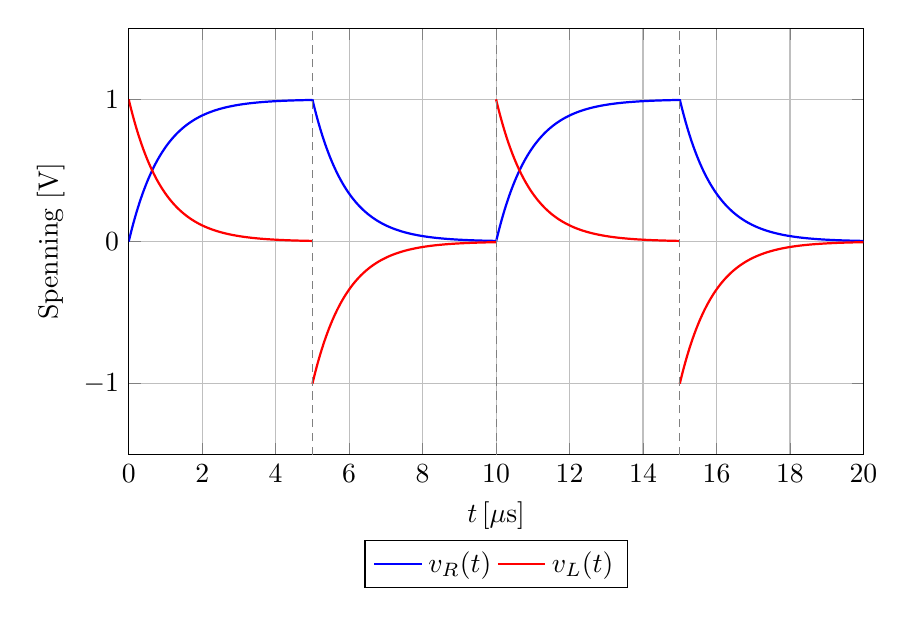
\begin{tikzpicture}
\begin{axis}[
    width=0.9\textwidth,
    height=7cm,
    xlabel={$t\,[\mathrm{\mu s}]$},
    ylabel={Spenning\ [V]},
    xmin=0, xmax=20,
    ymin=-1.5, ymax=1.5,
    grid=both,
    legend style={at={(0.5,-0.2)},anchor=north,legend columns=2},
    samples=200
]

    % Parametre (i mikrosekund): T = 10 µs, T/2 = 5 µs, tau ≈ 0.92 µs
    % v_R(t): spenning over motstanden
    % Periode 1: 0–10 µs
    \addplot[
        thick,
        blue,
        domain=0:5
    ]
        {1 - exp(-x/0.92)};              % 0 <= t < 5 us
    \addplot[
        thick,
        blue,
        domain=5:10,
        forget plot
    ]
        {exp(-(x-5)/0.92)};              % 5 <= t < 10 us
    % Periode 2: 10–20 µs
    \addplot[
        thick,
        blue,
        domain=10:15,
        forget plot
    ]
        {1 - exp(-(x-10)/0.92)};         % 10 <= t < 15 us
    \addplot[
        thick,
        blue,
        domain=15:20,
        forget plot
    ]
        {exp(-(x-15)/0.92)};             % 15 <= t < 20 us
    \addlegendentry{$v_R(t)$}

    % v_L(t): spenning over spolen
    % Periode 1: 0–10 µs
    \addplot[
        thick,
        red,
        domain=0:5
    ]
        {exp(-x/0.92)};                   % 0 <= t < 5 us
    \addplot[
        thick,
        red,
        domain=5:10,
        forget plot
    ]
        {-exp(-(x-5)/0.92)};              % 5 <= t < 10 us
    % Periode 2: 10–20 µs
    \addplot[
        thick,
        red,
        domain=10:15,
        forget plot
    ]
        {exp(-(x-10)/0.92)};              % 10 <= t < 15 us
    \addplot[
        thick,
        red,
        domain=15:20,
        forget plot
    ]
        {-exp(-(x-15)/0.92)};             % 15 <= t < 20 us
    \addlegendentry{$v_L(t)$}

    % Vertikale hjelpelinjer for T/2 og T
    \addplot[
        gray,
        densely dashed,
        forget plot
    ]
        coordinates {(5,-1.5) (5,1.5)};
    \addplot[
        gray,
        densely dashed,
        forget plot
    ]
        coordinates {(10,-1.5) (10,1.5)};
    \addplot[
        gray,
        densely dashed,
        forget plot
    ]
        coordinates {(15,-1.5) (15,1.5)};

\end{axis}
\end{tikzpicture}
\caption{Teoretisk spenning over spolen $L$ og motstanden $R$ for et firkantet inngangssignal med periode $T = 10\,\mathrm{\mu s}$ og tidskonstant $\tau \approx 0{,}92\,\mathrm{\mu s}$.}
\end{figure}

\noindent
Her ser vi hvordan disse to lagt til til resultere i firkantpulsen generert av funksjonsgeneratoren. Forskyvning i y aksen er riktig i forhold til resultatet vårt og skalering er riktig. Resultatet er ikke feil, men innstillingene for måling er ikke ideelle.



\subsection{Krets med RC-ledd}
Under ser vi kretsen med et kondensatorledd, og en graf for hva spenningskilden skal produsere.


\begin{figure}[H]\label{fig:krets-med-rc-ledd}
\centering
\begin{circuitikz}[american voltages]

    \node[circle, fill=black, inner sep=1.2pt] (BL)  at (0, 0)  {};
    \node[circle, fill=black, inner sep=1.2pt] (B)  at (5, 0)  {};
    \node[circle, fill=black, inner sep=1.2pt] (BR)  at (10, 0)  {};
    \node[circle, fill=black, inner sep=1.2pt] (TL)  at (0, 5)  {};
    \node[circle, fill=black, inner sep=1.2pt] (T)  at (5, 5)  {};
    \node[circle, fill=black, inner sep=1.2pt] (TR)  at (10, 5)  {};
    \node[circle, draw=black, fill=none, thick, inner sep=2pt] (VT)  at (12, 4)  {};
    \node[circle, draw=black, fill=none, thick, inner sep=2pt] (VB)  at (12, 1)  {};


    \node[above] at (T) {$A$};
    \node[ground] at (B) {};

    \node at (12, 3.5) {$+$};
    \node at (12, 1.5) {$-$};
    \node at (12, 2.5) {$v_0(t)$};

    \draw (TL) to[V=$v(t)$] (BL);
    \draw (TL) to[R=$2.2\text{k}\Omega$] (T);
    \draw (T) to[R=$3.9\text{k}\Omega$] (TR);
    \draw (TR) to[R, l_=$3.3\text{k}\Omega$] (BR);
    \draw (T) to[C, l_=$v_C(t)$, a^=$1\mu\text{F}$] (B);
    \draw (BL) -- (BR);

    \draw (10, 4) to[short, -] (VT);
    \draw (10, 1) to[short, -] (VB);
    


\end{circuitikz}
\caption{Kretsen i tilfelle 1}
\end{figure}

\noindent
Spenningskilden skal produsere slikt som i figur~\ref{fig:grafet_v_av_t} i teoridelen (samme figur grafet under).


\begin{figure}[H]
\centering
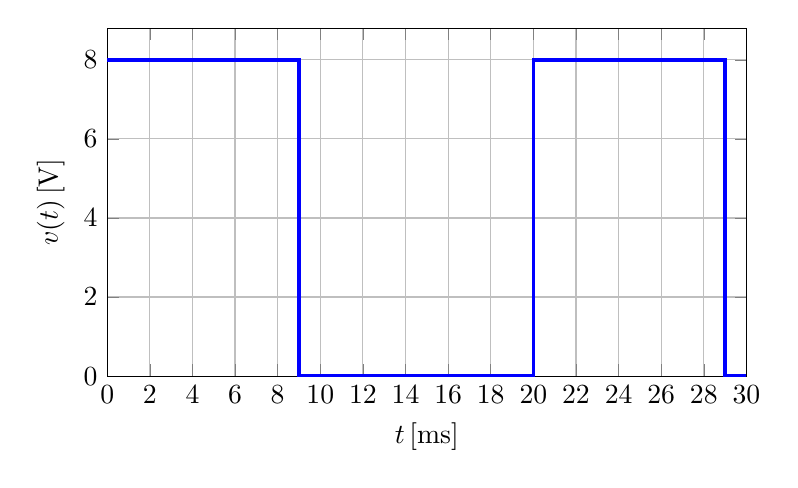
\begin{tikzpicture}
\begin{axis}[
    width=0.8\textwidth,
    height=6cm,
    xlabel={$t\,[\mathrm{ms}]$},
    ylabel={$v(t)\,[\mathrm{V}]$},
    xmin=0, xmax=30,
    ymin=0, ymax=8.8,
    ytick={0,2,4,6,8},
    xtick={0,2,...,30},
    grid=both
]
    \addplot[const plot, very thick, blue]
        coordinates {
            (0,8)
            (9,8)
            (9,0)
            (20,0)
            (20,8)
            (29,8)
            (29,0)
            (30,0)
        };
\end{axis}
\end{tikzpicture}
\caption{Inngangssignal $v(t)$ med høy-nivå $8\,\mathrm{V}$ i 9\,ms per periode.}
\end{figure}

\noindent
Resultatene for $v_C(t)$ og $v_0(t)$ er som under: